\documentclass[conference]{IEEEtran}
\IEEEoverridecommandlockouts
% The preceding line is only needed to identify funding in the first footnote. If that is unneeded, please comment it out.
\usepackage[nocompress]{cite}
\usepackage{amsmath,amssymb,amsfonts}
\usepackage{algorithmic}
\usepackage{graphicx}
\usepackage{textcomp}
\usepackage{xcolor}
\usepackage{booktabs}
\usepackage{url}
\usepackage{tikz}
\usetikzlibrary{positioning,arrows.meta,shapes.geometric,fit,backgrounds}
\usepackage{pgfplots}
\pgfplotsset{compat=1.18}
\usepackage{placeins}
\usepackage[hidelinks]{hyperref}
\def\BibTeX{{\rm B\kern-.05em{\sc i\kern-.025em b}\kern-.08em
    T\kern-.1667em\lower.7ex\hbox{E}\kern-.125emX}}
\begin{document}

\title{Higher-Order Accord Co-occurrence for Interaction-Free Perfume Recommendation}

\author{\IEEEauthorblockN{Azam Azri Ahmad}
\IEEEauthorblockA{\textit{Department of Electrical and Information Engineering} \\
\textit{Faculty of Engineering, Universitas Gadjah Mada}\\
Yogyakarta, Indonesia \\
azamazriahmad@mail.ugm.ac.id}
\and
\IEEEauthorblockN{Syukron Abu Ishaq Alfarozi}
\IEEEauthorblockA{\textit{Department of Electrical and Information Engineering} \\
\textit{Faculty of Engineering, Universitas Gadjah Mada}\\
Yogyakarta 55281, Indonesia \\
syukron.abu@ugm.ac.id}
\\
\IEEEauthorblockN{Bimo Sunarfri Hantono}
\IEEEauthorblockA{\textit{Department of Electrical and Information Engineering} \\
\textit{Universitas Gadjah Mada}\\
Yogyakarta, Indonesia \\
bhe@ugm.ac.id}
\and
\IEEEauthorblockN{Kuntpong Woraratpanya}
\IEEEauthorblockA{\textit{School of Information Technology} \\
\textit{King Mongkut's Institute of Technology Ladkrabang}\\
Bangkok, Thailand \\
kuntpong@it.kmitl.ac.th}
}

\maketitle

\begin{abstract}
Content-based perfume recommenders rank products by order-one accord similarity, such as
cosine or Jaccard over note sets, and treat accords as independent. Whether modeling how
accords \emph{co-occur} improves recommendation has not been tested under a leakage-free
protocol, and most product catalogs record no user interactions, which rules out the
collaborative and knowledge-graph recommenders that need an interaction signal. This paper
studies interaction-free, content-based perfume recommendation as a retrieval task: given a
reference perfume, a catalog is ranked to surface the product that imitates it, and a
held-out inspired-by edge supplies ground-truth relevance. The proposed matcher is
parameter-free; it extends accord TF-IDF with higher-order co-occurrence tokens---accord
pairs and triples---and its cosine score decomposes additively by interaction order, while
emitting auditable co-occurrence paths for explanation. On 340 products and 209 reference
perfumes under leave-one-out ranking, behind a three-source firewall whose query accords are
independently verified from Fragrantica, accuracy improves as co-occurrence order increases:
mean reciprocal rank rises from 0.454 for the order-one baseline to 0.508 at order three,
which outranks twelve comparators spanning marginal similarity, neural embeddings,
perceptual-taxonomy transport, and learned models. The gain is modest but statistically
robust, and higher-order structure carries the majority of the ranking signal. The
contribution is a finding and a leakage-free evaluation protocol rather than a new model.
\end{abstract}

\begin{IEEEkeywords}
recommender systems, content-based retrieval, co-occurrence, TF-IDF, explainability,
fragrance, non-circular evaluation
\end{IEEEkeywords}

\section{Introduction}
Aromatique is an Indonesian perfume brand that sells locally blended scents, many of them
crafted to smell like a well-known global perfume, across a growing network of branches.
During peak hours the recommendation load falls on the sales staff, who must match a
customer's reference scent to the right in-house product from memory; the brand needs an
automated recommender to relieve this bottleneck. Crucially, the catalog records only
content---each product's olfactory \emph{accords} (e.g., \textit{amber}, \textit{woody},
\textit{warm spicy}) and its family---and no clicks or ratings. The setting is therefore
\emph{interaction-free}: recommendations must be made from content alone.

Existing perfume recommenders are almost entirely content-based and \emph{order-one}: they
rank candidates by single-accord similarity using cosine over term frequency--inverse
document frequency (TF-IDF) vectors or Jaccard over accord sets. Lutan \cite{r23} surveys the
field, while Nurmuthia \textit{et al.} \cite{r24} and Fannisa \textit{et al.} \cite{r28} rely
on cosine, Jaccard, and TF-IDF over notes; none models how accords \emph{co-occur}. This is a
real limitation: two products can share the same individual accords with the reference yet
differ in which accords appear \emph{together}, so an order-one score ties the correct
imitation with a distractor, whereas higher-order structure separates them
(Fig.~\ref{fig:problem}).

Richer models are not directly available here. Interaction-driven recommenders that exploit
co-occurrence and higher-order connectivity---collaborative filtering, LightGCN, KGIN, and
KGAT \cite{r18,r19,r20}---report strong gains, but only in session or multi-behavior settings
\cite{r1,r2,r3,r4,r5}; they learn from a user--item signal this catalog does not contain.
Neural and learned embeddings, and perceptual-geometry priors from odor science
\cite{r10,r11,r12,r13}, are likewise attractive in principle, yet on small, imbalanced data
simple baselines routinely match or beat flexible models that overfit \cite{r14,r15,r16,r17}.
Whether accord \emph{co-occurrence} helps a content-only, interaction-free recommender---and
how far the benefit extends with interaction order---has not been tested under an evaluation
that cannot leak the answer.

\begin{figure}[t]
\centering
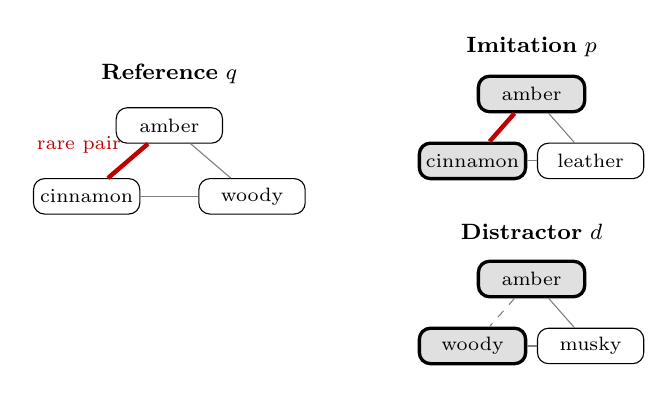
\begin{tikzpicture}[
  font=\footnotesize,
  acc/.style={draw, rounded corners, minimum width=1.35cm, minimum height=4.5mm,
              inner sep=1pt, font=\scriptsize, fill=white},
  sh/.style={draw, rounded corners, minimum width=1.35cm, minimum height=4.5mm,
             inner sep=1pt, font=\scriptsize, fill=black!12, very thick},
  rare/.style={ultra thick, red!75!black},
  common/.style={gray, dashed}]
% Reference q (left)
\node at (0,1.85) {\textbf{Reference} $q$};
\node[acc] (qa) at (0,1.2) {amber};
\node[acc] (qc) at (-1.05,0.3) {cinnamon};
\node[acc] (qw) at (1.05,0.3) {woody};
\draw[gray] (qa)--(qw); \draw[gray] (qc)--(qw);
\draw[rare] (qa)--(qc);
\node[red!75!black] at (-1.15,0.95) {\scriptsize rare pair};
% Imitation p (upper right)
\node at (4.6,2.2) {\textbf{Imitation} $p$};
\node[sh] (pa) at (4.6,1.6) {amber};
\node[sh] (pc) at (3.85,0.75) {cinnamon};
\node[acc] (pl) at (5.35,0.75) {leather};
\draw[gray] (pa)--(pl); \draw[gray] (pc)--(pl);
\draw[rare] (pa)--(pc);
% Distractor d (lower right)
\node at (4.6,-0.15) {\textbf{Distractor} $d$};
\node[sh] (da) at (4.6,-0.75) {amber};
\node[sh] (dw) at (3.85,-1.6) {woody};
\node[acc] (dm) at (5.35,-1.6) {musky};
\draw[gray] (da)--(dm); \draw[gray] (dw)--(dm);
\draw[common] (da)--(dw);
\end{tikzpicture}
\caption{Why higher order helps. Both the correct imitation $p$ and a distractor $d$ share two
individual accords with the reference $q$ (shaded), so an order-one score ties them. Only $p$
reproduces $q$'s rare co-occurring pair \textit{amber--cinnamon} (bold); $d$ shares only the
common \textit{amber--woody} pairing (dashed). Higher-order tokens therefore break the tie in
favor of the true imitation.}
\label{fig:problem}
\end{figure}

This paper takes a deliberately simple route: it extends accord TF-IDF with
\emph{higher-order} co-occurrence tokens---accords, accord pairs, and accord triples, the
subsets of a fragrance's accord set---weighted by inverse document frequency and compared by
cosine, so the score decomposes additively by interaction order. The matcher carries no
trained parameters, which on a catalog this small is a design choice rather than a limitation,
since added capacity only overfits. The contribution is a \emph{finding and a protocol}, not a
new model, at a moderate applied scope:
\begin{itemize}
\item \textbf{Finding.} Accord co-occurrence improves interaction-free perfume retrieval over
the order-one baseline; the gain strengthens with interaction order and then saturates, so we
adopt order three as the operating point.
\item \textbf{Protocol.} A non-circular, leakage-free evaluation with a three-source firewall
(local item accords, externally sourced query accords, and held-out imitation labels used only
as ground truth), under which we also explain why interaction-based recommenders such as KGAT
cannot be compared on this data.
\end{itemize}

\section{Problem Formulation and Non-circular Protocol}\label{sec:problem}

\subsection{Task and interaction order}
Let $\mathcal{P}=\{p_1,\dots,p_M\}$ be the catalog of local products, $M=340$; each product
$p$ has an accord set $A(p)\subseteq\mathcal{V}$ and a family label, where $\mathcal{V}$ is
the accord vocabulary. Let $\mathcal{Q}$ be the set of reference perfumes (branded
originals); each reference $q$ has accords $A(q)$. The imitation relation gives a
ground-truth set
\begin{equation}
g(q)=\{\,p\in\mathcal{P}\;:\;\textit{inspired\_by}(p)=q\,\}, \label{eq:gold}
\end{equation}
the products built to smell like $q$. A method scores every product, $s(q,p)$, ranks the
whole catalog, and is judged by the rank of the ground-truth product. Of the $340$ products,
$243$ carry a label and $97$ are unlabeled originals kept as genuine distractors; $209$
references have at least one labeled product and form the leave-one-out evaluation set.

The key quantity is \emph{interaction order}, the content-only analogue of the high-order
connectivity exploited by knowledge-graph recommenders \cite{r20}. The order-$k$ tokens of a
fragrance $f$ are its accord subsets of size $k$,
\begin{equation}
T_k(f)=\{\,S\subseteq A(f)\;:\;|S|=k\,\}, \label{eq:order}
\end{equation}
so order one is the single accords (marginal similarity), order two the co-occurring pairs,
and order three the co-occurring triples. A representation of order $N$ uses all tokens of
order $1\le k\le N$.

\subsection{Deployment versus evaluation}
The deployed recommender and the benchmark share an \emph{identical} scoring engine and
differ only in query source and in whether a ground-truth answer exists. In deployment the
query is a customer's free preference and any product may be returned---an in-house imitation
or an original. In evaluation the query is a reference perfume, because only there does a
held-out answer exist (the imitation edge); a reference perfume is never itself returned,
since the pool is the local catalog. The $97$ originals without a labeled imitation are thus
not discarded but retained in the pool as \emph{non-target} candidates, which makes the
retrieval realistically hard.

\subsection{A non-circular firewall}
The central methodological risk is circularity: if query features were copied from the
products they must retrieve, accord overlap would be a tautology. A three-source separation
guards against this (Table~\ref{tab:firewall}): item accords come from the local catalog,
query accords are sourced independently from Fragrantica ($264$ of $266$ \texttt{source\_url}
entries resolve to perfume-specific pages), and the imitation label is held out. Formally,
interaction-based recommenders (LightGCN, KGIN, KGAT) require a user--item matrix
$R\in\{0,1\}^{U\times I}$; here $U=\varnothing$, so $R$ is undefined and such models cannot be
instantiated. A leakage audit finally strips identity-bearing text before any text-based
method sees it: the reference name never appears, and distinctive name tokens found in the
free text of $32$ of $340$ products are removed.

\begin{table}[t]
\caption{Non-circular three-source firewall and dataset statistics}
\begin{center}
\begin{tabular}{lll}
\toprule
\textbf{Component} & \textbf{Source} & \textbf{Independent of} \\
\midrule
Item features  & local catalog accords              & the label \\
Query features & Fragrantica accords (external)     & local catalog \& label \\
Label          & held-out \textit{inspired\_by} edge & accord similarity \\
\midrule
\multicolumn{3}{l}{\footnotesize $340$ products ($243$ labeled $+\,97$ non-target), $209$ references,} \\
\multicolumn{3}{l}{\footnotesize $56$ shared accords; $264/266$ query source URLs verified on Fragrantica.} \\
\bottomrule
\end{tabular}
\label{tab:firewall}
\end{center}
\end{table}

\section{Method}\label{sec:method}
The matcher represents a fragrance by its accords \emph{and} by which accords co-occur in it,
weights every token by rarity, and compares two fragrances with a single cosine that splits
additively by interaction order. It has no trained parameters. Fig.~\ref{fig:pipeline} shows
the pipeline.

\subsection{Higher-order token representation}
Using the order-$k$ tokens of \eqref{eq:order}, the order-$N$ representation of a fragrance
$f$ pools all tokens up to order $N$,
\begin{equation}
T_{\le N}(f)=\bigcup_{k=1}^{N} T_k(f). \label{eq:tokens}
\end{equation}
Order one recovers the single accords of a plain TF-IDF baseline; orders two and three add the
co-occurring pairs and triples this work contributes.

\subsection{Weighting, normalization, and scoring}
Each token is weighted by inverse document frequency over the $M=340$ products, with document
frequency $\mathrm{df}(t)=|\{f:t\in T_{\le N}(f)\}|$:
\begin{equation}
\mathrm{idf}(t)=\log\frac{1+M}{1+\mathrm{df}(t)}+1. \label{eq:idf}
\end{equation}
Rare co-occurrences receive a high weight while ubiquitous single accords receive a low one, so
the hub penalty is automatic and parameter-free. A fragrance becomes a sparse vector $v_f$ with
$v_f[t]=\mathrm{idf}(t)$ for $t\in T_{\le N}(f)$ and $0$ otherwise, then $L_2$-normalized,
\begin{equation}
\hat v_f = v_f/\lVert v_f\rVert_2. \label{eq:vector}
\end{equation}
The score of a product $p$ for a reference $q$ is the cosine of the normalized vectors, which
separates exactly into per-order contributions,
\begin{equation}
s(q,p)=\langle \hat v_q,\hat v_p\rangle=\sum_{k=1}^{N} S_k(q,p), \label{eq:score}
\end{equation}
where the order-$k$ term aggregates the shared order-$k$ tokens,
\begin{equation}
S_k(q,p)=\frac{1}{\lVert v_q\rVert\,\lVert v_p\rVert}\sum_{t\in T_k(q)\cap T_k(p)}\mathrm{idf}(t)^2. \label{eq:terms}
\end{equation}
Ranking the $340$ products by $s(q,p)$ and taking the highest few gives the recommendations.
For the order-three method, the order-three term supplies on average $54\%$ of the top-ranked
score, order two $37\%$, and order one only $9\%$: higher-order structure carries the majority
of the signal.

\begin{figure}[t]
\centering
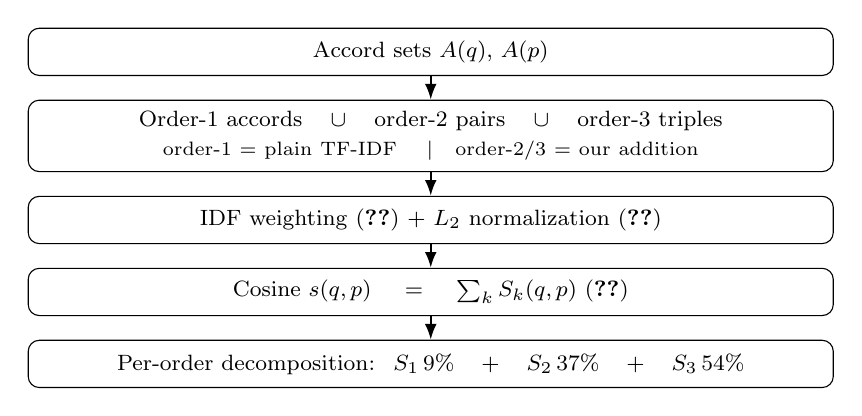
\begin{tikzpicture}[
  font=\footnotesize,
  box/.style={draw, rounded corners, align=center, text width=0.82\linewidth,
              inner sep=4pt, minimum height=6mm},
  arr/.style={-{Latex[length=2mm]}, thick}]
\node[box] (a) {Accord sets $A(q)$, $A(p)$};
\node[box, below=3mm of a] (t) {Order-1 accords $\;\cup\;$ order-2 pairs $\;\cup\;$ order-3 triples\\[1pt]
{\scriptsize order-1 $=$ plain TF-IDF \quad$|$\quad order-2/3 $=$ our addition}};
\node[box, below=3mm of t] (w) {IDF weighting~\eqref{eq:idf} $+$ $L_2$ normalization~\eqref{eq:vector}};
\node[box, below=3mm of w] (c) {Cosine $s(q,p)=\sum_k S_k(q,p)$~\eqref{eq:score}};
\node[box, below=3mm of c] (d) {Per-order decomposition:\; $S_1\,9\%\;+\;S_2\,37\%\;+\;S_3\,54\%$};
\draw[arr] (a)--(t); \draw[arr] (t)--(w); \draw[arr] (w)--(c); \draw[arr] (c)--(d);
\end{tikzpicture}
\caption{Scoring pipeline. Accords are expanded into higher-order co-occurrence tokens
(order one reproduces plain TF-IDF; orders two and three are the contribution),
IDF-weighted and $L_2$-normalized, and compared by a cosine whose value decomposes by
interaction order. Percentages are the average share of the top-ranked score.}
\label{fig:pipeline}
\end{figure}

\subsection{Parameter-free design and explanations}
The matcher has no trained weights, so it cannot overfit---a principled choice on a catalog
with a single relevant product per query, where added capacity is later shown to degrade
accuracy. As a byproduct, the shared higher-order tokens of a recommendation, grouped by
Edwards-wheel super-family \cite{r10}, form auditable co-occurrence paths (\texttt{kg\_paths})
for a downstream explanation layer, in the spirit of path-based explainable recommendation
\cite{r21}; we report them as an artifact, not a faithfulness claim.

\section{Experiments}\label{sec:experiments}
We ask three research questions:\\
\textbf{RQ1:} Does accord co-occurrence (order $\ge 2$) improve retrieval over the order-one
baseline?\\
\textbf{RQ2:} How far does the improvement continue with interaction order---is there a
saturation point?\\
\textbf{RQ3:} How does the order-three matcher compare with established paradigms: marginal
similarity, neural embeddings, perceptual transport, and learned models?

\subsection{Setup}
The dataset and its non-circular firewall are summarized in Table~\ref{tab:firewall}; accord
lists are parsed by splitting on commas and semicolons, lower-casing, and trimming. The
order-$N$ matcher is compared against twelve methods spanning four paradigms: \emph{marginal}
similarity (Jaccard, TF-IDF cosine, BM25); \emph{neural} embeddings (multilingual
Sentence-BERT \cite{r22}, Word2Vec over accords, node2vec over the co-occurrence graph);
\emph{perceptual} transport (a tree-Wasserstein distance over the Edwards wheel \cite{r10},
following graph-based optimal transport \cite{r7,r9});
and \emph{learned} models (a PPMI--SVD embedding, a signature-subgraph ranker, a per-bigram
salience logistic model, a low-rank bilinear metric, and a gradient-boosting fusion). B2
(TF-IDF cosine) is the primary baseline. With one relevant product per query, quality is
measured by mean reciprocal rank (MRR) and Hits@$k$,
\begin{align}
\mathrm{MRR}&=\frac{1}{|\mathcal{Q}|}\sum_{q}\frac{1}{r_q},\\
\mathrm{Hits}@k&=\frac{1}{|\mathcal{Q}|}\sum_{q}\mathbf{1}[\,r_q\le k\,],\label{eq:metrics}
\end{align}
where $r_q$ is the rank of the ground-truth product and ties use the expected reciprocal rank
under uniform tie-breaking. All methods rank the full pool of $340$ products under
leave-one-out over the $209$ queries; learned rankers are scored out-of-fold with $5$-fold
GroupKFold grouped by query, and stochastic methods are averaged over $5$ seeds
(mean$\pm$std). Significance uses the Wilcoxon signed-rank test paired across queries on
reciprocal ranks, with $95\%$ confidence intervals from $10{,}000$ bootstrap resamples; the
text-based method is run after the leakage audit of Section~\ref{sec:problem}.

\subsection{RQ1 and RQ2: co-occurrence helps, then saturates}
Adding co-occurrence tokens raises accuracy sharply and then plateaus
(Fig.~\ref{fig:ablation}). MRR climbs from $0.454$ at order one to $0.496$ at order two and
$0.508$ at order three, and both steps are statistically significant (order one to two,
$p=8.7\times10^{-8}$; order two to three, $\Delta\mathrm{MRR}=0.012$, $p=2.8\times10^{-3}$). Beyond order three the curve is flat:
order four is not significantly better than order three ($\Delta\mathrm{MRR}=0.003$, $95\%$
CI $[-0.010,+0.005]$), so we adopt order three as the operating point. The plateau has a
simple cause: high-order co-occurrences become vanishingly rare, so little is left to
exploit---a query and its target share on average $4.1$ four-way, $1.2$ five-way, and $0.3$
six-way accord combinations, against $7.7$ triples. This makes the saturation point
dataset-dependent: a catalog with richer accord lists could extend the useful order.

\begin{figure}[t]
\centering
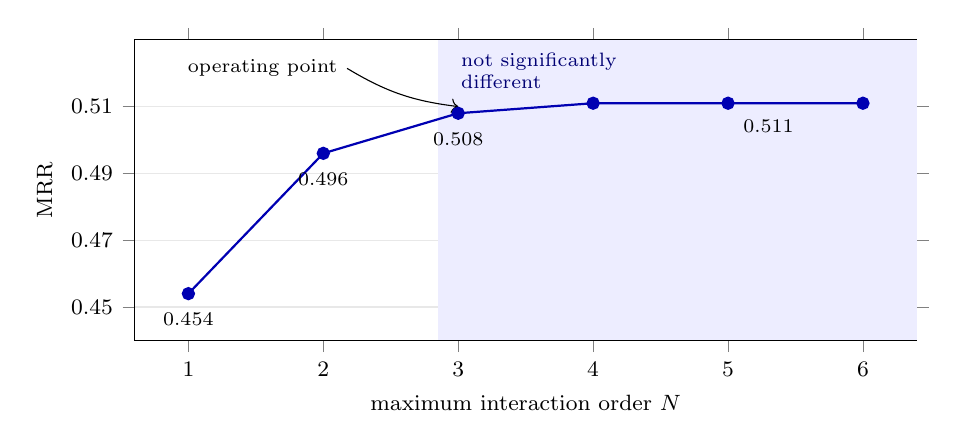
\begin{tikzpicture}
\begin{axis}[width=0.95\linewidth,height=5.4cm,font=\footnotesize,
  xlabel={maximum interaction order $N$}, ylabel={MRR},
  xmin=0.6,xmax=6.4, ymin=0.44, ymax=0.53,
  xtick={1,2,3,4,5,6}, ytick={0.45,0.47,0.49,0.51},
  ymajorgrids, grid style={gray!18}, tick align=outside, clip=false]
% plateau band: orders 3-6 are not significantly different
\fill[blue!7] (axis cs:2.85,0.44) rectangle (axis cs:6.4,0.53);
\node[font=\scriptsize, text=blue!45!black, align=left, anchor=north west]
  at (axis cs:2.95,0.529) {not significantly\\different};
% curve
\addplot[thick, mark=*, color=blue!70!black] coordinates
 {(1,0.454)(2,0.496)(3,0.508)(4,0.511)(5,0.511)(6,0.511)};
% value labels (below the markers)
\node[anchor=north, font=\scriptsize] at (axis cs:1,0.451) {0.454};
\node[anchor=north, font=\scriptsize] at (axis cs:2,0.493) {0.496};
\node[anchor=north, font=\scriptsize] at (axis cs:3,0.505) {0.508};
\node[anchor=north, font=\scriptsize] at (axis cs:5.3,0.509) {0.511};
% operating-point annotation above the curve, leader to N=3
\node[font=\scriptsize, anchor=south] (op) at (axis cs:1.55,0.516) {operating point};
\draw[->,thin] (op.east) to[bend right=12] (axis cs:3,0.510);
\end{axis}
\end{tikzpicture}
\caption{Retrieval accuracy versus maximum interaction order. Accuracy rises steeply from
order one to two, again to order three, and then flattens. Although order four attains a
marginally higher point estimate, it is not significantly better than order three
($\Delta$MRR $=0.003$, $95\%$ CI $[-0.010,+0.005]$); order three is adopted as the operating
point.}
\label{fig:ablation}
\end{figure}

\subsection{RQ3: order three versus established paradigms}
Table~\ref{tab:main} places order three against all twelve comparators. It ranks first on
every metric and beats each comparator significantly ($p<0.01$ throughout); the headline
margin over the marginal baseline B2 is $\Delta\mathrm{MRR}=+0.054$ ($p=5.6\times10^{-9}$).
Two regimes of margin stand apart. Over the simple, near-marginal methods the win is real but
small---$+0.054$ over TF-IDF (B2), $+0.064$ over PPMI--SVD (A2), $+0.051$ over gradient
boosting (A6), and $+0.080$ over Jaccard (B1)---so these methods approach without surpassing
the co-occurrence signal. Over the complex models the win is decisive: $+0.236$ over
Sentence-BERT (B4), $+0.323$ over Word2Vec (B5), $+0.358$ over the bilinear metric (A5), and
$+0.369$ over per-bigram salience (A4). Tellingly, the two parametric models that explicitly
try to \emph{learn} co-occurrence weights---per-bigram salience and the bilinear metric---overfit
the worst and collapse to the bottom of the table under the one-positive-per-query imbalance.
Exact, unweighted co-occurrence thus beats \emph{learned} co-occurrence here, which is why the
parameter-free form is a design decision, not a limitation. The weak Sentence-BERT result is
only partial evidence against neural semantics: query and product text are asymmetric---sparse
accord lists against rich Indonesian prose---so B4 is penalized by a text mismatch independent
of its semantic quality.

\begin{table}[t]
\caption{Order three versus twelve comparators (leave-one-out; stochastic methods
mean$\pm$std over 5 seeds). Bold marks the method of record.}
\begin{center}\footnotesize\setlength{\tabcolsep}{4pt}
\begin{tabular}{llccc}
\toprule
\textbf{ID} & \textbf{Method} & \textbf{MRR} & \textbf{H@1} & \textbf{H@3} \\
\midrule
\textbf{O3} & \textbf{order-3 co-occurrence} & \textbf{0.508} & \textbf{0.397} & \textbf{0.567} \\
\midrule
\multicolumn{5}{l}{\textit{Marginal}} \\
B1 & Jaccard            & 0.428 & 0.303 & 0.487 \\
B2 & TF-IDF cosine      & 0.454 & 0.335 & 0.507 \\
B3 & BM25               & 0.388 & 0.278 & 0.433 \\
\multicolumn{5}{l}{\textit{Neural embedding}} \\
B4 & Sentence-BERT      & 0.272 & 0.163 & 0.311 \\
B5 & Word2Vec           & 0.185{\scriptsize\,$\pm$0.011} & 0.110 & 0.182 \\
B6 & node2vec           & 0.340{\scriptsize\,$\pm$0.013} & 0.233 & 0.371 \\
\multicolumn{5}{l}{\textit{Perceptual transport}} \\
A1 & Edwards tree-W.\    & 0.284 & 0.174 & 0.306 \\
\multicolumn{5}{l}{\textit{Learned}} \\
A2 & PPMI--SVD          & 0.444{\scriptsize\,$\pm$0.001} & 0.343 & 0.498 \\
A3 & signature LTR      & 0.433{\scriptsize\,$\pm$0.006} & 0.303 & 0.500 \\
A4 & bigram salience    & 0.139{\scriptsize\,$\pm$0.012} & 0.060 & 0.145 \\
A5 & bilinear metric    & 0.150{\scriptsize\,$\pm$0.027} & 0.072 & 0.150 \\
A6 & GBM fusion         & 0.457{\scriptsize\,$\pm$0.010} & 0.325 & 0.533 \\
\bottomrule
\multicolumn{5}{l}{\scriptsize Std shown for MRR; omitted for Hits due to space.}
\end{tabular}
\label{tab:main}
\end{center}
\end{table}

A concrete case makes the mechanism visible (Fig.~\ref{fig:case}). For the reference
\textit{Burberry Woman}, the correct Aromatique product \textit{Zimba} is retrieved at rank
one not merely because they share individual accords but because they share a rare accord
\emph{triple} such as \textit{fruity--sweet--vanilla}; a distractor carrying \textit{fruity},
\textit{sweet}, or \textit{vanilla} in isolation does not reproduce this co-occurring
signature.

\begin{figure}[t]
\centering
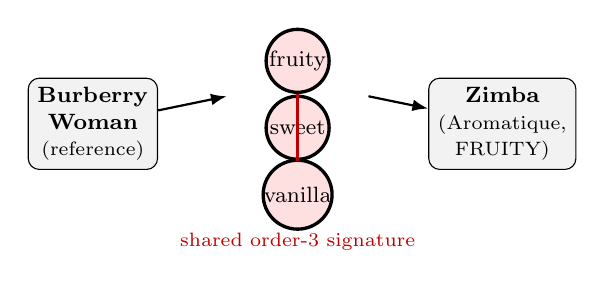
\begin{tikzpicture}[font=\footnotesize,
  ref/.style={draw, rounded corners, align=center, fill=black!5},
  prod/.style={draw, rounded corners, align=center, fill=black!5},
  tri/.style={draw, circle, minimum size=8mm, inner sep=0pt, fill=red!12, very thick},
  arr/.style={-{Latex[length=2mm]}, thick}]
\node[ref] (q) at (0,0) {\textbf{Burberry}\\\textbf{Woman}\\{\scriptsize(reference)}};
\node[tri] (t1) at (2.6,0.8) {fruity};
\node[tri] (t2) at (2.6,-0.05) {sweet};
\node[tri] (t3) at (2.6,-0.9) {vanilla};
\draw[red!75!black,very thick] (t1)--(t2)--(t3)--(t1);
\node[prod] (p) at (5.2,0) {\textbf{Zimba}\\{\scriptsize(Aromatique,}\\{\scriptsize FRUITY)}};
\draw[arr] (q) -- (1.7,0.35);
\draw[arr] (3.5,0.35) -- (p);
\node[red!75!black, font=\scriptsize] at (2.6,-1.5) {shared order-3 signature};
\end{tikzpicture}
\caption{Case study. The reference \textit{Burberry Woman} and its correct imitation
\textit{Zimba} share a rare accord triple such as \textit{fruity--sweet--vanilla}; this
order-three co-occurrence, not the individual accords, lifts the true product to rank one.}
\label{fig:case}
\end{figure}

\FloatBarrier
\section{Conclusion}\label{sec:conclusion}
This work studied interaction-free, content-based perfume recommendation and asked whether
modeling accord co-occurrence improves retrieval over the marginal similarity that dominates
the field. The contribution is a finding and a protocol, not a new model. The task is cast as
retrieval behind a non-circular evaluation---a three-source firewall with externally verified
query accords, a leakage audit, and a comparison against twelve methods across four
paradigms---and the reason interaction-driven recommenders (KGAT, LightGCN, KGIN) cannot be
instantiated on a catalog without user interactions is made explicit. Within this protocol, a
deliberately parameter-free matcher that pools accord co-occurrences up to order three ranks
first, beating every comparator; accuracy rises with interaction order and then saturates, so
order three is the operating point. The headline gain over the TF-IDF baseline is modest but
robust ($\Delta\mathrm{MRR}=+0.054$, $p=5.6\times10^{-9}$), and higher-order structure carries
most of the signal (order three alone supplies $54\%$ of the top-ranked score). Adding a
learning-to-rank layer over this representation yields no significant improvement ($p=0.18$),
so the parameter-free form is retained.

The result is reported with its limits intact. The effect is modest in absolute terms, and all
data come from a single proprietary catalog in one market, so external validity remains
untested. Accords are binary, without per-accord intensity, so products with identical accord
sets cannot be distinguished, and because the imitation relation is a perceptual proxy rather
than a measure of user satisfaction, its already high query--target accord overlap---about
$86\%$---imposes a ceiling intrinsic to the task that bounds the achievable gain. The advantage
across paradigms is, to our knowledge, the first non-circular demonstration of its kind, yet it
is claimed only for this setting, and the high-order plateau itself reflects the scarcity of
shared high-order tokens in this catalog and may shift with richer accord vocabularies. These
limits point to natural next steps: intensity-weighted co-occurrence, a symmetric-text
evaluation to isolate the semantic contribution of sentence encoders, a counterfactual
edge-ablation study to quantify the faithfulness of the exported \texttt{kg\_paths}, and
replication across further catalogs and domains.

\bibliographystyle{IEEEtran}
\bibliography{references}

\end{document}
